%======================================================================
%  Thesis background notes: LLM inference on HBM-equipped CPUs
%  Build from this directory with:
%      tectonic --keep-logs --keep-intermediates --reruns 1 notes.tex
%======================================================================
\documentclass[11pt,a4paper]{article}

\usepackage[margin=2.6cm]{geometry}
\usepackage[T1]{fontenc}
\usepackage{lmodern}
\usepackage{microtype}
\usepackage{amsmath}
\usepackage{amssymb}
\usepackage{graphicx}
\usepackage{booktabs}
\usepackage{tabularx}
\usepackage{array}
\usepackage{xcolor}
\usepackage{enumitem}
\usepackage{caption}
\usepackage{float}
\usepackage{flafter}
\usepackage{placeins}
\usepackage{tikz}
\usetikzlibrary{arrows.meta, positioning, fit, calc}
\usepackage{listings}
\usepackage{xurl}
\usepackage[numbers,sort&compress]{natbib}
\usepackage[colorlinks=true, linkcolor=accent, urlcolor=accent,
            citecolor=accent]{hyperref}

\definecolor{accent}{RGB}{128,0,32}
\definecolor{hbmcol}{RGB}{213,125,28}
\definecolor{ddrcol}{RGB}{55,105,165}
\definecolor{neutralcol}{RGB}{235,238,242}

\newcolumntype{Y}{>{\raggedright\arraybackslash}X}
\setlist[itemize]{leftmargin=*, itemsep=2pt, topsep=4pt}
\setlist[enumerate]{leftmargin=*, itemsep=2pt, topsep=4pt}
\captionsetup{font=small, labelfont=bf}
\setlength{\emergencystretch}{2em}
\widowpenalty=10000
\clubpenalty=10000

\lstdefinestyle{shell}{
  language=bash,
  basicstyle=\ttfamily\footnotesize,
  backgroundcolor=\color{neutralcol},
  frame=single,
  rulecolor=\color{black!25},
  framerule=0.4pt,
  columns=fullflexible,
  keepspaces=true,
  breaklines=true,
  showstringspaces=false,
  aboveskip=8pt,
  belowskip=8pt
}

\title{\textbf{Technical Background and Experimental Rationale}\\[5pt]
       \Large LLM Inference on HBM-Equipped CPUs\\[3pt]
       \large The CRESCO8 Xeon Max Platform}
\author{Lucian Crainic}
\date{26 July 2026}

\begin{document}
\maketitle

\begin{abstract}
\noindent
These notes establish the technical background for a thesis on large
language model inference on CPUs with on-package High Bandwidth Memory
(HBM).  They describe the Xeon Max memory hierarchy and the CRESCO8
testbed, develop a performance model for prefill and autoregressive
decode, and critically synthesize the relevant measurement literature.
The central experimental comparison is local HBM versus local DDR5 on
the same processor in Flat mode; comparisons with other processors are
secondary because they change several variables at once.  Particular
attention is given to working-set capacity, arithmetic intensity, NUMA
placement, and the distinction between theoretical capability and
measured behaviour.  The final part turns these concepts into a focused,
reproducible experimental design that can be incorporated into the
background and methodology chapters of the thesis.
\end{abstract}

\tableofcontents

\clearpage
\part{Experimental platform}
%======================================================================
%  Hardware platform: SD650 V3 and Intel Xeon CPU Max
%======================================================================

\section{Xeon Max and the SD650 V3}
\label{sec:xeon-max-platform}

\subsection{The unit of analysis}

The Lenovo ThinkSystem SD650~V3 is a dense, direct-water-cooled server
tray rather than a single compute node.  One tray contains two
independent dual-socket nodes, and six trays fit in a 6U DW612S
enclosure~\cite{lp1603}.  This distinction matters when reporting
quantities: the CRESCO8 allocation is a \emph{node}; memory locality is
defined first at the \emph{socket}; and the scheduler may allocate
individual cores within the node.

\begin{table}[tbp]
\centering
\small
\caption{Hardware hierarchy and the properties relevant to this study.
Product capability is separated from the installed CRESCO8
configuration described in Section~\ref{sec:cresco8}
~\cite{lp1603,cresco8doc}.}
\label{tab:hardware-hierarchy}
\begin{tabularx}{\textwidth}{@{}lYY@{}}
\toprule
\textbf{Level} & \textbf{Composition} & \textbf{Relevance} \\
\midrule
DW612S enclosure
  & Six SD650~V3 trays (12 independent nodes)
  & Shared power and cooling infrastructure; not an allocation unit. \\
SD650~V3 tray
  & Two independent dual-socket nodes
  & High-density packaging; the two nodes do not form one shared-memory
    system. \\
Compute node
  & Two Xeon processors connected by Intel UPI
  & Scheduler allocation and the largest cache-coherent NUMA system used
    by the single-node experiments. \\
Xeon Max socket
  & CPU cores, 64\,GB on-package HBM2e and eight DDR5 channels
  & Primary locality domain and the cleanest unit for comparing HBM with
    DDR5. \\
\bottomrule
\end{tabularx}
\end{table}

The product guide covers several processor, memory, storage and network
options.  Most of those options are irrelevant to the thesis.  The
important configuration is the Xeon CPU Max 9480 installed on CRESCO8:
56 physical cores per socket, 64\,GB of HBM2e, eight DDR5-4800 channels,
and four UPI links~\cite{intel9480,lp1603}.  A two-socket node therefore
provides 112 physical cores and 128\,GB of nominal HBM capacity.  The
node also contains DDR5, but its installed capacity and channel
population are properties of CRESCO8, not of the product family.

\begin{figure}[tbp]
\centering
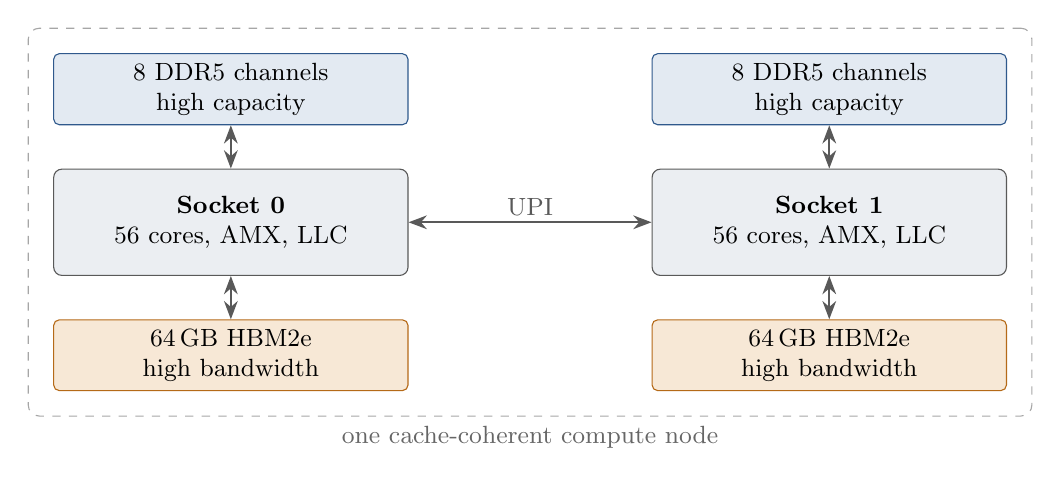
\begin{tikzpicture}[
  font=\small,
  socket/.style={draw=black!65, fill=neutralcol, rounded corners=3pt,
                 minimum width=4.5cm, minimum height=1.35cm,
                 align=center},
  hbm/.style={draw=hbmcol!85!black, fill=hbmcol!18, rounded corners=2pt,
              minimum width=4.5cm, minimum height=0.85cm, align=center},
  ddr/.style={draw=ddrcol!85!black, fill=ddrcol!14, rounded corners=2pt,
              minimum width=4.5cm, minimum height=0.85cm, align=center},
  link/.style={{Stealth}-{Stealth}, thick, black!65}
]
  \node[socket] (s0) at (-3.8,0)
    {\textbf{Socket 0}\\56 cores, AMX, LLC};
  \node[socket] (s1) at (3.8,0)
    {\textbf{Socket 1}\\56 cores, AMX, LLC};
  \node[hbm, below=0.55cm of s0] (h0)
    {64\,GB HBM2e\\high bandwidth};
  \node[hbm, below=0.55cm of s1] (h1)
    {64\,GB HBM2e\\high bandwidth};
  \node[ddr, above=0.55cm of s0] (d0)
    {8 DDR5 channels\\high capacity};
  \node[ddr, above=0.55cm of s1] (d1)
    {8 DDR5 channels\\high capacity};

  \draw[link] (s0) -- node[above, fill=white, inner sep=2pt]{UPI} (s1);
  \draw[link] (s0) -- (h0);
  \draw[link] (s1) -- (h1);
  \draw[link] (s0) -- (d0);
  \draw[link] (s1) -- (d1);

  \node[draw=black!35, dashed, rounded corners=4pt, inner sep=9pt,
        fit=(d0)(d1)(h0)(h1),
        label={[black!60]below:{one cache-coherent compute node}}] {};
\end{tikzpicture}
\caption{Conceptual locality map of a CRESCO8 Xeon Max node.  Each
socket has local HBM and DDR5; access to the other socket traverses UPI.
The diagram represents locality, not physical package routing.
Author's synthesis based on the platform and cluster documentation
~\cite{lp1603,cresco8doc}.}
\label{fig:node-locality}
\end{figure}

\subsection{Compute capability: AMX does not remove the memory problem}

Xeon Max is a Sapphire Rapids processor with conventional x86 cores,
AVX-512, and Intel Advanced Matrix Extensions (AMX).  AMX adds per-core
tile registers and matrix-multiply instructions for BF16 and INT8
operands~\cite{intelmax,na2024llmcpu}.  It can substantially accelerate
matrix operations with suitable shapes and kernels, especially the
large matrix--matrix products encountered during prompt processing.
There is no native INT4 AMX dot-product instruction; low-bit runtimes
must unpack, dequantize, or use specialized integer kernels.  Whether a
model benefits from AMX therefore depends on the runtime, data format,
packing scheme and matrix dimensions.

Peak instruction throughput is not an application result.  Small
matrices, batch-one matrix--vector operations, packing overhead and
memory stalls can leave the matrix units underused.  Likewise, the
advertised maximum turbo frequency is a single-core limit, not the
frequency of a socket executing sustained AMX kernels.  Frequency,
package power and throttling state must be observed during experiments
rather than inferred from specification tables.

\subsection{The memory hierarchy}
\label{sec:memory-hierarchy}

HBM and DDR5 trade different resources.  HBM provides much greater
aggregate bandwidth and 64\,GB of nominal capacity per socket.  DDR5
provides substantially more capacity and can have lower unloaded access
latency.  HBM is therefore not simply ``faster memory'': it is most
valuable when a workload issues enough concurrent requests to approach
its bandwidth and when the bandwidth-critical working set is placed
locally.

Published STREAM results illustrate both the advantage and the need for
local measurement.  Na et al.\ report 588\,GB/s for HBM and
233.8\,GB/s for DDR5 on a Xeon Max 9468 socket
~\cite{na2024llmcpu}.  Ibeid et al.\ report 680--840\,GB/s for HBM and
235--245\,GB/s for DDR5 on a related Xeon Max 9470C
~\cite{ibeid2025aurora}.  These sustained values are 2.5--3.4 times
apart, but the HBM results themselves differ by more than 15\%.  SKU,
clustering mode, thread placement and benchmark configuration are
plausible causes.  None of these numbers should be used as the bandwidth
of CRESCO8 before the Max 9480 nodes are measured.

Three paths must be distinguished in every result:

\begin{itemize}
  \item \textbf{local HBM or local DDR5}, reached from cores on the same
        socket;
  \item \textbf{remote memory}, reached through UPI from the other
        socket; and
  \item \textbf{mixed placement}, in which pages, threads or model
        objects span several locality domains.
\end{itemize}

An apparently node-wide 128\,GB HBM allocation is consequently two
64\,GB local tiers.  A workload uses the aggregate capacity and
bandwidth only if data and computation are balanced across sockets.

\subsection{HBM memory modes}
\label{sec:hbm-modes}

Xeon Max supports three ways to expose HBM
~\cite{lp1603,intelmaxtuning}.  The mode is selected in firmware and is
normally fixed for the lifetime of a boot.

\begin{figure}[tbp]
\centering
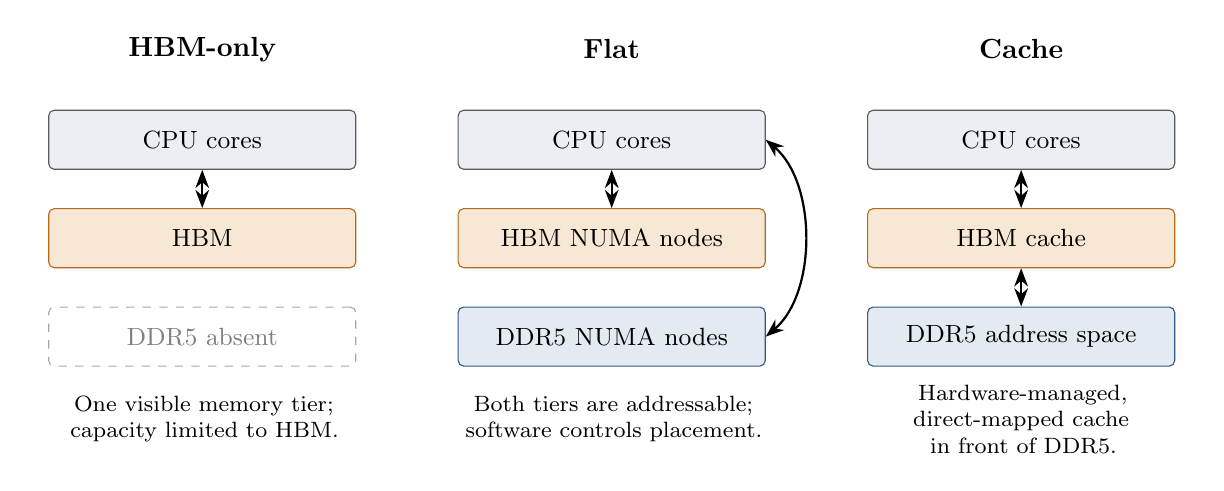
\begin{tikzpicture}[
  font=\small,
  cpu/.style={draw=black!65, fill=neutralcol, rounded corners=2pt,
              minimum width=3.9cm, minimum height=0.75cm, align=center},
  hbm/.style={draw=hbmcol!85!black, fill=hbmcol!18, rounded corners=2pt,
              minimum width=3.9cm, minimum height=0.75cm, align=center},
  ddr/.style={draw=ddrcol!85!black, fill=ddrcol!14, rounded corners=2pt,
              minimum width=3.9cm, minimum height=0.75cm, align=center},
  absent/.style={draw=black!35, dashed, text=black!50, rounded corners=2pt,
                 minimum width=3.9cm, minimum height=0.75cm, align=center},
  link/.style={{Stealth}-{Stealth}, thick},
  note/.style={font=\footnotesize, text width=4.2cm, align=center}
]
  \node[font=\bfseries] at (0,1.15) {HBM-only};
  \node[cpu] (c0) at (0,0) {CPU cores};
  \node[hbm] (h0) at (0,-1.25) {HBM};
  \node[absent] (d0) at (0,-2.5) {DDR5 absent};
  \draw[link] (c0) -- (h0);
  \node[note] at (0,-3.55)
    {One visible memory tier; capacity limited to HBM.};

  \node[font=\bfseries] at (5.2,1.15) {Flat};
  \node[cpu] (c1) at (5.2,0) {CPU cores};
  \node[hbm] (h1) at (5.2,-1.25) {HBM NUMA nodes};
  \node[ddr] (d1) at (5.2,-2.5) {DDR5 NUMA nodes};
  \draw[link] (c1) -- (h1);
  \draw[link] (c1.east) .. controls +(0.65,-0.55) and
                                  +(0.65,0.55) .. (d1.east);
  \node[note] at (5.2,-3.55)
    {Both tiers are addressable; software controls placement.};

  \node[font=\bfseries] at (10.4,1.15) {Cache};
  \node[cpu] (c2) at (10.4,0) {CPU cores};
  \node[hbm] (h2) at (10.4,-1.25) {HBM cache};
  \node[ddr] (d2) at (10.4,-2.5) {DDR5 address space};
  \draw[link] (c2) -- (h2);
  \draw[link] (h2) -- (d2);
  \node[note] at (10.4,-3.55)
    {Hardware-managed, direct-mapped cache in front of DDR5.};
\end{tikzpicture}
\caption{The three Xeon Max memory modes, shown for one socket.  Flat
mode is the only mode that exposes HBM and DDR5 as separately
controllable memory tiers.  Author's synthesis from the Xeon Max product
and tuning guides~\cite{lp1603,intelmaxtuning}.}
\label{fig:hbm-modes}
\end{figure}

\begin{description}
  \item[HBM-only mode.] The system contains no DDR5 and exposes HBM as
  ordinary system memory.  It is simple for software but imposes a hard
  capacity limit.  It is not the documented CRESCO8 configuration.

  \item[Flat mode.] HBM and DDR5 share the physical address space but
  appear as distinct NUMA memory nodes.  Applications can allocate
  directly from a tier, or an external policy can bind pages with
  \texttt{mbind}, libnuma or \texttt{numactl}.  Allocation is not enough:
  first touch, page migration and memory mapping can change actual page
  residency, which must be verified.

  \item[Cache mode.] HBM is a hardware-managed, direct-mapped cache in
  front of DDR5.  Applications see the DDR5 capacity without placing
  objects explicitly, but software cannot choose which objects remain
  in HBM.  Conflict misses, warm state and a working set near the cache
  capacity can make performance workload-dependent
  ~\cite{ibeid2025aurora}.
\end{description}

Flat mode provides the strongest experimental design because local HBM
and local DDR5 can be compared on the same socket without changing the
processor or executable.  A Flat-versus-Cache comparison answers a
different question: it measures explicit placement against a hardware
cache policy.

\subsection{Clustering and NUMA}

Memory mode is independent of the processor's clustering mode.  In
Quadrant mode, one socket is normally presented as one compute locality
domain.  Sub-NUMA Clustering (SNC4) exposes four domains per socket,
each associated with a subset of cores, cache, DDR channels and HBM.
SNC4 can increase bandwidth and reduce local latency for software that
places workers and data per quadrant, but it also makes remote accesses
easier to create.  In Flat+SNC4, the nominal 64\,GB HBM socket is divided
into four 16\,GB locality domains.

This distinction explains why a mode cannot be labelled universally
``best''.  Ibeid et al.\ obtain the highest STREAM bandwidth with SNC4
and explicit locality, whereas Na et al.\ observe worse inference
performance and more remote traffic under SNC4
~\cite{ibeid2025aurora,na2024llmcpu}.  The result depends on the
software's placement policy, not only on the processor setting.

\subsection{Cooling and instrumentation}

Direct water cooling allows two high-power processors to operate in a
dense node, but it does not guarantee a fixed frequency or energy
efficiency.  The relevant quantities are measured socket frequency,
temperature, package power and throttling state.  Product-guide claims
about facility heat recovery or cooling savings are not evidence about
inference performance.

The SD650~V3 includes XClarity management and a TI INA226-based
power/energy meter with 100\,Hz sampling capability
~\cite{lp1603}.  This establishes a platform capability, not user
access on CRESCO8.  Intel RAPL, management-controller telemetry and
whole-node power meters cover different system boundaries; they must
not be combined without first validating their scope, units, sampling
and permissions.

\subsection{Consequences for the thesis}

The hardware background yields four requirements for the experimental
work:

\begin{enumerate}
  \item identify the active memory and clustering modes from the
        allocated node rather than from the product guide;
  \item measure sustained local HBM and DDR5 behaviour before using a
        Roofline or interpreting inference results;
  \item bind both threads and pages, then verify page residency and
        remote traffic; and
  \item record frequency, thermal and power state so that a placement
        effect is not confused with a change in operating conditions.
\end{enumerate}

%======================================================================
%  CRESCO8 as the experimental testbed
%======================================================================

\section{CRESCO8 as the experimental testbed}
\label{sec:cresco8}

\subsection{Documented configuration}

CRESCO8 is the current CRESCO system at the ENEA research centre in
Portici.  It entered service in 2025 and is connected by a 200\,Gb/s
Mellanox NDR fabric~\cite{cresco8doc,eneapress}.  The operational user
page distinguishes three compute-node classes:

\begin{table}[tbp]
\centering
\small
\caption{CRESCO8 node classes documented by ENEAGRID.  Counts describe a
dated operational document, not a permanent scheduler inventory
~\cite{cresco8doc}.}
\label{tab:cresco8-node-classes}
\begin{tabularx}{\textwidth}{@{}lcccY@{}}
\toprule
\textbf{Class} & \textbf{Nodes} & \textbf{CPU cores/node}
 & \textbf{Memory/node} & \textbf{Processor or accelerator} \\
\midrule
CPU
 & 760 & 128 & 512\,GB DDR5
 & 2$\times$ Xeon Platinum 8592+ \\
CPU--HBM
 & 15 & 112 & 1,024\,GB DDR5 + 128\,GB HBM
 & 2$\times$ Xeon CPU Max 9480 \\
GPU
 & 17 & 128 & 512\,GB DDR5 + accelerator HBM
 & 2$\times$ Xeon Platinum 8592+ and
   4$\times$ Intel Data Center GPU Max 1550 \\
\bottomrule
\end{tabularx}
\end{table}

The same page calls this a 793-node system, although the listed classes
sum to 792 and its reported core total is consistent with the 792-node
breakdown.  Earlier commissioning material gives yet another snapshot
~\cite{eneacresco8slides}.  This inconsistency is operational rather
than scientific: every experiment should retain dated
\texttt{sinfo -N} and \texttt{scontrol show node} output, and the thesis
should report the observed inventory rather than silently reconcile
historical documents.

\FloatBarrier

\subsection{Why the HBM partition supports a clean comparison}

Each documented HBM node contains two Max 9480 sockets, 1\,TB of DDR5
and 128\,GB of HBM.  This makes three comparisons possible, but they do
not have equal evidential strength:

\begin{enumerate}
  \item \textbf{Local HBM versus local DDR5 on the same Max 9480
        socket} is the primary comparison.  Processor, core count,
        executable and most firmware conditions can be held constant.

  \item \textbf{One socket versus two sockets, or Quadrant versus SNC4},
        tests the runtime's response to topology.  It is a placement
        experiment, not a pure memory-technology comparison.

  \item \textbf{Max 9480 versus Platinum 8592+} is a secondary
        system-level baseline.  The processors differ in generation,
        core count, cache, clocks, memory channels and uncore behaviour.
        The contrast cannot identify an HBM effect by itself.
\end{enumerate}

The installed DDR capacity does not reveal the DIMM layout.  Sixteen
64\,GB DIMMs would populate all channels, but the platform also permits
eight 128\,GB DIMMs with Xeon Max~\cite{lp1603}.  Channel population,
memory frequency and local bandwidth therefore require direct
inspection.  The presence of DDR5 also means that the nodes use Flat or
Cache mode rather than the no-DDR HBM-only configuration, but the ENEA
page does not identify which mode is active.  In Flat mode, HBM appears
as memory-only NUMA nodes; in Cache mode it does not appear separately.

The NDR link has a raw one-direction rate of 25\,GB/s per node, far
below local HBM bandwidth.  Multi-node inference may still be necessary
for capacity, but communication can then dominate the placement effect.
Single-node experiments should establish a stable result before adding
distributed parallelism.

\subsection{Scheduler and storage context}

The documented production partition is \texttt{cresco8\_hbm}, with 14
nodes and a 24-hour limit; \texttt{cresco8\_hbm\_dbg} lists two nodes
and a one-hour limit~\cite{cresco8doc}.  Their hostnames can overlap, so
these counts must not be added.

Compute nodes are reached only through Slurm.  The front ends are for
editing, compilation and submission, not benchmarking.  ENEAGRID
provides AFS for shared home directories and Lustre for parallel I/O;
large model files and benchmark output belong on the latter, subject to
the site's current mount points and quotas.  Compiler, MPI and profiler
modules listed on the web page are useful starting points, but an
experiment must record the modules and linked libraries actually loaded
on the run date.

\subsection{First allocation: capture facts before benchmarking}
\label{sec:first-allocation}

The first HBM allocation should create a machine-readable system
manifest.  The following script is deliberately a topology-capture
skeleton rather than a performance benchmark; account names, available
utilities and Slurm resource syntax must be checked on the live system.

\begin{lstlisting}[style=shell,
  caption={Minimal exclusive allocation for a CRESCO8 topology
  manifest.}]
#!/bin/bash
#SBATCH --nodes=1
#SBATCH --ntasks=1
#SBATCH --cpus-per-task=112
#SBATCH --partition=cresco8_hbm
#SBATCH --exclusive
#SBATCH --hint=nomultithread
#SBATCH --output=%j-system.txt

set -u

echo "job_id=${SLURM_JOB_ID}"
echo "host=$(hostname)"
date --iso-8601=seconds
scontrol show job "${SLURM_JOB_ID}"
lscpu
lscpu --extended
numactl --hardware
lstopo-no-graphics 2>/dev/null || true
cat /sys/devices/system/cpu/smt/active 2>/dev/null || true
findmnt -t lustre 2>/dev/null || true
module list 2>&1 || true
\end{lstlisting}

The manifest should be extended, subject to permissions, with the
following evidence:

\begin{table}[tbp]
\centering
\small
\caption{Minimum platform record for an inference result.}
\label{tab:platform-record}
\begin{tabularx}{\textwidth}{@{}lY@{}}
\toprule
\textbf{Category} & \textbf{Record} \\
\midrule
Identity
 & Hostname, Slurm job ID, partition, date and node allocation. \\
Processor
 & Exact SKU, sockets, physical cores, SMT state, microcode, governor,
   turbo policy and observed frequency. \\
Memory
 & Memory and clustering modes, NUMA distance matrix, HBM and DDR
   node IDs, DIMM population, huge-page state and measured local/remote
   bandwidth. \\
I/O
 & Lustre mount and striping used for model loading; NIC identity and
   NUMA affinity if multi-node tests are attempted. \\
Software
 & OS and kernel, loaded modules, compiler, runtime commit, linked
   libraries, build flags and complete command line. \\
Telemetry
 & Available RAPL, performance-counter and management-controller
   interfaces, including permissions and measurement boundaries. \\
\bottomrule
\end{tabularx}
\end{table}

This separation between documented configuration and observed
configuration is important.  Vendor documents establish what the
platform can support, and ENEAGRID describes a dated cluster state.
Only the archived manifest establishes the conditions under which a
reported result was obtained.


\clearpage
\part{Workload model and research evidence}
%======================================================================
%  Workload concepts and analytical model
%======================================================================

\section{A performance model for LLM inference}
\label{sec:inference-model}

\subsection{Prefill and autoregressive decode}

Inference for a decoder-only transformer has two phases
~\cite{na2024llmcpu}.  During
\emph{prefill}, the model processes the prompt and constructs the
initial key--value (KV) cache.  Tokens from the prompt can be processed
in parallel, so the linear layers often form comparatively large matrix
multiplications.  During \emph{decode}, the model generates one new
token per sequence at each iteration.  Each iteration requires the
relevant weights and KV state, then appends the key and value for the new
token.  Dense full-context attention reads the prior cached KV; sliding
window or sparse attention can reduce that history.

\begin{figure}[tbp]
\centering
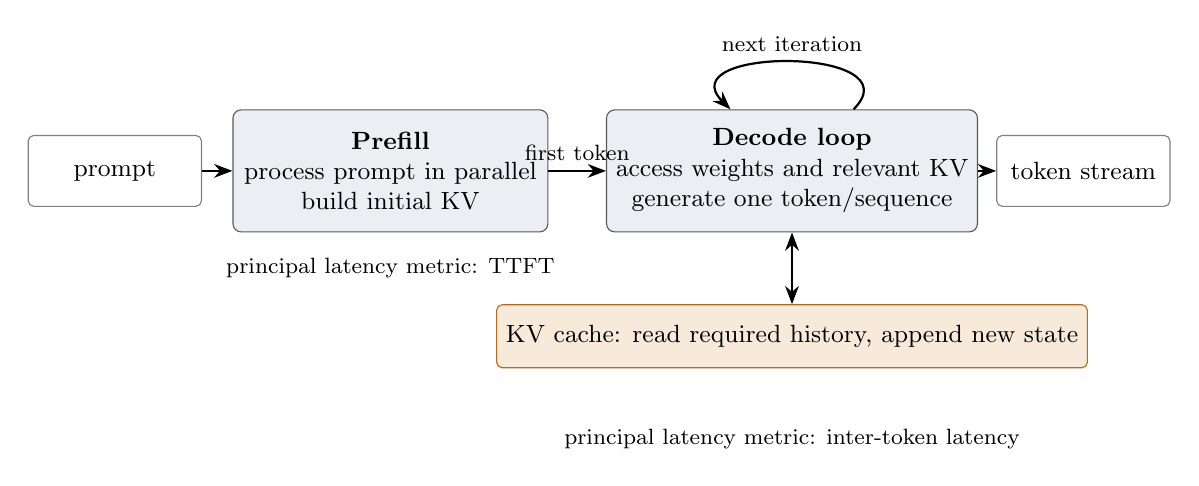
\begin{tikzpicture}[
  font=\small,
  io/.style={draw=black!50, fill=white, rounded corners=2pt,
             minimum width=2.2cm, minimum height=0.9cm, align=center},
  phase/.style={draw=black!65, fill=neutralcol, rounded corners=3pt,
                minimum width=4.0cm, minimum height=1.55cm, align=center},
  kv/.style={draw=hbmcol!85!black, fill=hbmcol!16, rounded corners=2pt,
             minimum width=4.0cm, minimum height=0.8cm, align=center},
  flow/.style={-{Stealth}, thick},
  note/.style={font=\footnotesize, align=center}
]
  \node[io] (prompt) at (-6.0,0) {prompt};
  \node[phase] (prefill) at (-2.5,0)
    {\textbf{Prefill}\\process prompt in parallel\\build initial KV};
  \node[phase] (decode) at (2.6,0)
    {\textbf{Decode loop}\\access weights and relevant KV\\
     generate one token/sequence};
  \node[io] (output) at (6.3,0) {token stream};
  \node[kv] (cache) at (2.6,-2.1)
    {KV cache: read required history, append new state};

  \draw[flow] (prompt) -- (prefill);
  \draw[flow] (prefill) -- node[above, note]{first token} (decode);
  \draw[flow] (decode) -- (output);
  \draw[flow, {Stealth}-{Stealth}] (decode) -- (cache);
  \draw[flow] (decode.45) .. controls +(0.8,0.8) and +(-0.8,0.8)
       .. (decode.135) node[midway, above, note]{next iteration};

  \node[note, below=0.2cm of prefill]
    {principal latency metric: TTFT};
  \node[note, below=0.65cm of cache]
    {principal latency metric: inter-token latency};
\end{tikzpicture}
\caption{Dataflow of prompt prefill and autoregressive decode.  The
frequent description of prefill as compute-bound and decode as
bandwidth-bound is a useful first-order model, not a universal property:
batch, context, precision and kernel implementation can change the
regime.  Author's synthesis.}
\label{fig:prefill-decode}
\end{figure}

This phase distinction is essential when evaluating HBM.  A single
end-to-end throughput number can hide a faster decode phase behind a
long prompt, or hide a prefill regression behind a long generation.
TTFT and decode latency must therefore be reported separately.  Prefill
usually offers matrix--matrix parallelism, whereas low-batch decode is
closer to matrix--vector execution and repeatedly streams weights.
Larger batches increase weight reuse and can move decode toward
matrix-engine throughput; long contexts simultaneously increase KV
traffic.

\FloatBarrier

\subsection{Working-set capacity}
\label{sec:working-set}

For a model with \(P\) parameters and a stored weight precision of
\(q_w\) bits, the first-order weight footprint is

\[
  M_W = P\frac{q_w}{8} + M_{\mathrm{format}},
\]

where \(M_{\mathrm{format}}\) includes scales, zero-points, alignment,
and any prepacked or duplicated representation created by the runtime.
The model file size is not necessarily the resident weight footprint.

For \(B\) concurrent sequences, cached length \(S\), \(L\) transformer
layers, \(H_{\mathrm{KV}}\) KV heads, head dimension \(d_h\), and
\(q_{\mathrm{KV}}\) bits per cached element, the KV footprint is

\[
  M_{\mathrm{KV}} =
  2 B S L H_{\mathrm{KV}} d_h \frac{q_{\mathrm{KV}}}{8}.
\]

The factor two accounts for keys and values.  Grouped-query and
multi-query attention reduce the KV footprint because
\(H_{\mathrm{KV}}\) is smaller than the number of query heads.  The
complete resident set is

\[
  M_{\mathrm{live}} =
  M_W + M_{\mathrm{KV}} + M_{\mathrm{activations}}
  + M_{\mathrm{workspace}} + M_{\mathrm{runtime}}.
\]

This arithmetic identifies where capacity boundaries may occur, but the
boundary must use the OS-exposed NUMA capacity on the allocated node and
a measured safety margin.  The advertised 64\,GB per socket is not a
usable-allocation guarantee: system use, allocator fragmentation and
workspace consume part of it.  A node may expose roughly 128\,GB across
two sockets, but that capacity is not uniformly local; using it requires
a placement strategy that distributes data and execution deliberately.

Quantization changes both sides of the experiment.  Fewer bits reduce
weight capacity and memory traffic, potentially reducing the benefit of
HBM for a model that already fits.  At the same time, quantization can
move a larger model below the HBM capacity boundary and remove DDR or
remote traffic altogether.  Packing, dequantization and kernel coverage
prevent performance from scaling exactly with bit width.  Weight and KV
precision must therefore be reported separately.

\subsection{Arithmetic intensity and the Roofline bound}
\label{sec:roofline}

The Roofline model relates arithmetic intensity \(I=F/D\), measured in
FLOP/byte, to compute throughput and memory bandwidth
~\cite{williams2009roofline}:

\[
  P_{\mathrm{attainable}}
  \leq
  \min\!\left(P_{\mathrm{compute}},
              I B_{\mathrm{effective}}\right).
\]

For one inference step, a corresponding lower-bound model is

\[
  T_{\mathrm{step}}
  \gtrsim
  \max\!\left(
      \frac{F_{\mathrm{step}}}{P_{\mathrm{effective}}},
      \frac{D_{\mathrm{step}}}{B_{\mathrm{effective}}}
  \right)
  + T_{\mathrm{communication}} + T_{\mathrm{runtime}}.
\]

The effective quantities must be measured for the selected kernel,
placement and core count.  Processor peak FLOP/s and theoretical pin
bandwidth are ceilings, not values to substitute uncritically.

For a dense linear layer during decode, if a stored weight is used once
for each of \(B\) sequences in a batch, a useful first-order
approximation is

\[
  I_{\mathrm{weights}} \approx \frac{2B}{b_w}
  \quad \text{FLOP/byte},
\]

where \(b_w\) is the stored bytes per weight and a multiply--add is
counted as two FLOPs.  The approximation assumes that each fetched dense
weight is reused across the \(B\) sequences.  At batch one, BF16 weight
streaming is therefore close to one FLOP/byte before KV,
activation and runtime traffic are included.  Batching reuses weights
and raises arithmetic intensity, which explains why HBM is expected to
matter most for low-batch decode and why AMX can become more important
as the matrix dimensions grow.

This model also clarifies why bandwidth alone is insufficient:

\begin{itemize}
  \item \textbf{Bandwidth} sets the rate for many concurrent,
        sufficiently regular memory requests.
  \item \textbf{Latency} sets the cost of a dependent or lightly loaded
        access path.  HBM can have higher unloaded latency than DDR5
        while sustaining much greater bandwidth under load
        ~\cite{ibeid2025aurora}.
  \item \textbf{Capacity} determines whether the critical working set
        remains local.  Crossing a 64\,GB socket boundary can introduce
        DDR5 or UPI traffic and cause a discontinuity that a simple
        single-tier Roofline does not predict.
\end{itemize}

For concurrent HBM and DDR5 traffic, a no-contention service-time
estimate can range from perfect overlap to serialization of the
per-tier transfers.  It is not a general bound: shared uncore resources,
cache conflicts, UPI traffic and memory-controller interference can make
the measured time worse than the serialized estimate.  Simultaneous
HBM--DDR traffic must therefore be characterized before a tiered
placement policy is modelled.

\subsection{Placement is part of the algorithm}

In Flat mode the operating system exposes memory tiers through NUMA,
but it does not know which model objects are bandwidth-critical.
Several mechanisms can therefore produce the wrong placement:
allocator first touch, worker migration, memory-mapped model pages,
automatic NUMA balancing, and a runtime that creates prepacked copies
after the initial allocation.  A command-line memory policy is evidence
of intent, not evidence of residency.

The relevant experimental object is consequently not ``the model in
HBM'' but a verified mapping between:

\begin{itemize}
  \item worker threads and physical cores;
  \item weight, KV, activation and workspace pages and their NUMA nodes;
  \item local or remote memory traffic observed during each inference
        phase; and
  \item the time interval used for performance and energy measurement.
\end{itemize}

This mapping is also the basis for testing topology-aware execution.
Independent replicas can use one local socket each; a single model can
be sharded across sockets or SNC domains; and selected objects can be
placed in different memory tiers.  These designs answer different
questions and should not be grouped under a generic ``two-socket run''.

\subsection{Metrics and boundaries}

For \(O\) generated tokens in a synchronous request,

\[
  T_{\mathrm{E2E}}
  =
  T_{\mathrm{TTFT}} +
  \sum_{j=2}^{O} T_{\mathrm{ITL},j}.
\]

At minimum, results should report TTFT, median and tail ITL, end-to-end
latency, output tokens/s and requests/s.  The report must state whether
tokenization, model loading, queueing and warm-up are included.  Static
batch throughput and online serving goodput are different constructs:
the latter additionally depends on arrivals, scheduling and declared
latency objectives.

Hardware counters are explanatory measurements rather than performance
metrics.  HBM and DDR traffic, UPI traffic, memory-controller
utilization, cache misses, achieved frequency and AMX-related counters
can support a mechanism only when their collection overhead,
multiplexing and scope are documented.

\subsection{Predictions to test}

The model yields three bounded predictions:

\begin{enumerate}
  \item local HBM should benefit low-batch decode more than compute-dense
        prefill, but the speedup need not equal the STREAM bandwidth
        ratio;
  \item performance should change when the verified live set crosses a
        local HBM boundary, with the size and direction of the change
        depending on placement and memory mode; and
  \item batching and lower-bit weights should reduce weight-bandwidth
        pressure, while long contexts can reintroduce pressure through
        the KV cache.
\end{enumerate}

These statements are hypotheses.  The literature reviewed next
motivates them but does not establish them for CRESCO8.

%======================================================================
%  Critical literature review and research gap
%======================================================================

\section{Related work and the research gap}
\label{sec:related-work}

\subsection{Corpus and source roles}

The supplied file
\texttt{Lessons from HPL and HPL-MxP on Aurora.pdf} now contains the
intended Goto et al.\ paper, \emph{Sustaining Exascale Performance:
Lessons from HPL and HPL-MxP on Aurora}, arXiv:2604.09517v1
~\cite{goto2026aurorahpl}.  Its title, authors and deployment results
were checked against the local twelve-page copy.

The four sources answer different parts of the argument.  Na et
al.\ provide the closest LLM workload precedent
~\cite{na2024llmcpu}; Ibeid et al.\ isolate memory bandwidth, latency,
mode and locality effects~\cite{ibeid2025aurora}; Goto et al.\ show the
importance of explicit tier staging and resource mapping at production
scale
~\cite{goto2026aurorahpl}; and Dongarra et al.\ provide architectural
motivation rather than a directly comparable baseline
~\cite{dongarra2026gpus}.  Their transfer limits are addressed with the
results below rather than treating the four works as equivalent
evidence.

\subsection{Na et al.: the closest inference precedent}
\label{sec:na-review}

Na et al.\ evaluate Intel Extension for PyTorch (IPEX) on a dual-socket
Xeon Max 9468 server and compare it with a previous-generation Xeon and
with single A100 and H100 GPUs running FlexGen
~\cite{na2024llmcpu}.  Their main comparisons bind one 48-core Max
socket; only the core-count sweep extends to 96 cores.  The CPU
experiments use BF16 OPT and LLaMA-2 models, prompt length 128,
generation length 32 and batch sizes from 1 to 32; a separate sweep
increases the prompt length.  This is the closest platform and workload
match in the corpus, but its results need careful qualification.

\begin{table}[H]
\centering
\small
\caption{Results from Na et al.\ and the interpretation used here
~\cite{na2024llmcpu}.}
\label{tab:na-findings}
\begin{tabularx}{\textwidth}{@{}YYY@{}}
\toprule
\textbf{Reported result} & \textbf{What it supports}
 & \textbf{What it does not establish} \\
\midrule
Depending on batch, Xeon Max geometric-mean throughput over the tested
models is 3.2--6.3$\times$ that of the Ice Lake system.
 & Matrix acceleration and the newer memory system make recent CPUs
   substantially more credible for inference.
 & A causal HBM or AMX speedup: cores, cache, DDR generation,
   microarchitecture and software paths also change. \\
\addlinespace[2pt]
Quadrant+Flat gives the best average of the four configurations under
the paper's HBM-first Flat placement.
 & In this setup, explicit HBM placement outperforms hardware-managed
   caching; unmanaged fine-grained NUMA is costly.
 & A universal preference for Quadrant mode.  Exact allocation,
   first-touch and binding details are not disclosed. \\
\addlinespace[2pt]
On average over the tested models and batches, 48 cores outperform a
naive 96-core execution.
 & Remote traffic can erase the value of additional cores.
 & An inherent one-socket scaling limit; replicas or topology-aware
   sharding are not evaluated. \\
\addlinespace[2pt]
At batch one, the CPU outperforms the tested FlexGen A100/H100 runs for
oversized models.
 & Capacity and data movement can dominate accelerator arithmetic at
   low batch.
 & General CPU superiority.  For LLaMA2-70B at batch 16 and prompt
   length at least 256, the offloaded H100 regains lower latency; when a
   model fits GPU memory, the GPUs are faster.  Multi-GPU serving is not
   tested. \\
\bottomrule
\end{tabularx}
\end{table}

The paper's GPU result is therefore best read as a data-movement result.
It compares direct CPU execution with a particular single-GPU
offloading system.  It does not compare like-for-like production
serving stacks.  The study also omits quantized weights, long
generations, energy, online arrivals, tail latency and output-quality
validation.  Repetition count, dispersion, complete software versions,
firmware, warm-up and the exact NUMA command are not reported.  Its
experimental design can be reimplemented, but the paper does not
support exact numerical reproduction.  It also proposes, without
implementing or evaluating, NUMA-aware hot/cold placement and
CPU--GPU layer partitioning.  A later placement contribution must
acknowledge that prior proposal.

\subsection{Ibeid et al.: bandwidth, latency and locality}
\label{sec:ibeid-review}

Ibeid et al.\ separate memory-system effects more clearly
~\cite{ibeid2025aurora}.  On the Borealis testbed they use Xeon Max
9470C processors and run STREAM, Intel Memory Latency Checker, PCIe and
MPI microbenchmarks, followed by three HPC applications chosen to stress
bandwidth, latency or capacity.  At the time of the study, production
Aurora was configured in Quadrant+Flat mode; the full single-socket
Flat/Cache and Quadrant/SNC4 matrix comes from Borealis.

\begin{table}[tbp]
\centering
\small
\caption{Single-socket STREAM Triad bandwidth on the Borealis Xeon Max
9470C testbed, in GB/s~\cite{ibeid2025aurora}.  The paper does not fully
specify array size, first touch or cache-state controls.}
\label{tab:ibeid-stream}
\begin{tabular}{@{}lccc@{}}
\toprule
 & \multicolumn{2}{c}{\textbf{Flat mode}} & \textbf{Cache mode} \\
\cmidrule(lr){2-3}
\textbf{Clustering} & \textbf{DDR5} & \textbf{HBM} & \textbf{DDR5+HBM cache} \\
\midrule
Quadrant, full socket & 235 & 680 & 560 \\
SNC4, full socket     & 245 & 840 & 575 \\
SNC4, one quadrant    &  60 & 210 & 150 \\
\bottomrule
\end{tabular}
\end{table}

In the two full-socket Flat-mode rows, HBM bandwidth is 2.9--3.4 times
DDR5 bandwidth, and SNC4 raises full-socket HBM bandwidth by about 24\%
over Quadrant.
However, unloaded latency favours DDR5: the paper reports 112.9\,ns for
Quadrant/DDR and 134.9\,ns for Quadrant/HBM.  Under increasing access
load, DDR5 saturates sooner while HBM sustains greater bandwidth before
latency rises sharply.  These results support a three-way distinction:
HBM for concurrent bandwidth demand, DDR5 for capacity and potentially
lower lightly loaded latency, and explicit locality for collecting the
available bandwidth.

Unless stated otherwise, Ibeid et al.\ repeat experiments three times
and report means; the latency study uses ten repetitions and reports a
mean and range.  Most other results do not report dispersion, and the
STREAM allocation and cache-state details remain insufficient for exact
reproduction.

The application results reinforce that there is no universal mode
ranking.  Explicit HBM performs best when a bandwidth-intensive working
set fits; Cache mode can help when the working set exceeds HBM; and DDR5
can remain preferable for lightly loaded latency-sensitive work.  Those
applications are not proxies for transformer inference.  They provide
mechanisms and measurements to reproduce, not a predicted LLM speedup.
Because Cache mode is direct-mapped, page-colour conflicts can also
change its result.  The paper uses page shuffling (``Fake NUMA'') to
mitigate such conflicts, so behaviour near 64\,GB must not be read as a
capacity-only effect.

\FloatBarrier

\subsection{The SNC4 result is software-dependent}
\label{sec:snc4-synthesis}

The two measurement papers appear to disagree.  Ibeid et al.\ obtain
their highest HBM bandwidth and several best application results with
SNC4 and explicit per-domain placement.  Na et al.\ find that both SNC4
configurations lose to Quadrant and report increased remote cache
traffic.  Both observations can hold: SNC4 exposes locality, but
software must align allocation and execution with that locality.

This is a productive gap rather than a contradiction in the hardware.
An MPI application can exploit SNC4 when ranks, pages and network
interfaces are explicitly bound per domain; MPI alone does not
guarantee locality.  Ibeid et al.\ recover an SNC4 MPI deficit through
explicit quadrant-to-interface mapping.  A shared-memory runtime that
allocates tensors without regard to the four domains can incur remote
traffic and smaller per-domain capacity.  CRESCO8 should therefore test
both a deliberately local SNC4 design and an unmanaged baseline if
administrators can expose that mode.

\subsection{Goto et al.: lessons from production scale}

Goto et al.\ report three production-scale Aurora campaigns, culminating in
1.012\,EF/s for FP64 HPL on 9,234 nodes, with 78.8\% parallel scaling
efficiency, and
11.64\,EF/s for mixed-precision HPL-MxP on 9,500 nodes
~\cite{goto2026aurorahpl}.  These values use different precision and are
not like-for-like throughput measurements.

The paper adds a relevant example of deliberate memory tiering.  Each
Aurora CPU has 64\,GB HBM2e and 512\,GB DDR5.  The global HPL matrix
remains in DDR because it exceeds HBM capacity, while tiles used for
panel factorisation, triangular solves and row exchange are staged into
HBM.  This demonstrates a production design that combines DDR capacity
with HBM for selected CPU-side operations.  Overall runtime is dominated
by GPU GEMM, and the paper does not ablate the staging policy, so it
does not quantify an HBM speedup transferable to LLM inference.

The study's second transferable lesson is that sustained performance
required
deterministic NUMA/PCIe-aware mapping, explicit CPU--GPU pipelining,
phase-specific communication choices and resilience to transient faults.
HPL-MxP improved from 10.6\,EF/s at ISC24 to 11.64\,EF/s at SC24,
about 9.8\%.  The authors identify AMX enablement as the primary
configuration change.  Their own impact table states that its
classifications are engineering assessments rather than controlled
ablations; the campaign comparison is therefore strong operational
evidence, not an isolated 9.8\% AMX measurement.

These findings support two methodological choices for this thesis:
resource mapping is part of the implementation, and a benchmark result
is credible only with a complete mapping and run manifest.  The paper
does not measure CPU-only LLM inference or isolate CPU HBM, so its
exascale throughput numbers should not appear as evidence for an HBM
speedup on CRESCO8.

\subsection{Dongarra et al.: architectural motivation, not a baseline}

Dongarra, Hoefler and Matsuoka argue that CPUs combining vector and
matrix engines, low-precision arithmetic and on-package HBM address the
three historical reasons for discrete GPU acceleration: arithmetic
throughput, memory bandwidth and data movement
~\cite{dongarra2026gpus}.  They retain an important boundary: GPUs
remain central to frontier-scale training, while HBM-equipped CPUs may
be attractive for inference and mixed irregular/dense scientific
workflows.

The manuscript's empirical discussion is asymmetric.  It summarizes a
companion study described as in preparation for arXiv: A64FX decode
results are measured, whereas results for a newer matrix-enhanced CPU,
including prefill and energy implications, are partly projected from
specifications.  Its trillion-parameter mixture-of-experts workload,
256K context and low-bit formats are also far from the CRESCO8 baseline.
Software maturity, energy and interconnect effects remain unresolved.
The manuscript therefore motivates the research question and the need
for runtime-aware placement, but it cannot substitute for measurements
on the Max 9480.

\subsection{What the literature establishes}

Taken together, the sources support four bounded conclusions:

\begin{enumerate}
  \item On-package HBM provides a large sustained bandwidth advantage
        over DDR5 on Xeon Max, but the achieved value depends on
        clustering and placement.
  \item Low-batch autoregressive decode is a strong candidate for
        bandwidth limitation, whereas larger prefill and batched decode
        can place more pressure on matrix throughput.
  \item Direct CPU inference can be competitive when the alternative
        repeatedly moves an oversized working set over PCIe; this is a
        capacity and data-movement claim, not a general CPU--GPU ranking.
  \item Topology results belong to the hardware--software combination.
        A poor two-socket or SNC4 result does not prove that the added
        resources are unusable.
\end{enumerate}

\subsection{What remains unanswered}
\label{sec:research-gap}

No source in the reviewed corpus performs a controlled, same-socket
comparison of local HBM and local DDR5 for modern quantized LLM
inference while separating prefill and sustained decode.  The following
questions remain unanswered by the reviewed corpus and require
measurement on CRESCO8:

\begin{itemize}
  \item how quantized weight and KV formats change the HBM benefit;
  \item what occurs when the verified live set approaches and crosses a
        64\,GB local HBM boundary;
  \item whether topology-aware sharding or independent replicas can
        reverse the reported SNC4 and two-socket regressions; and
  \item whether a performance gain also reduces energy per token under a
        clearly defined measurement boundary.
\end{itemize}

Answering the first three questions with a frozen runtime, raw data and
uncertainty is a sufficient and coherent thesis contribution.  Energy
is retained only if the measurement interface and boundary can be
validated.  GPU comparison, online serving and multi-node inference are
extensions rather than prerequisites.


\clearpage
\part{Experimental design}
%======================================================================
%  Focused experimental design
%======================================================================

\section{Focused experimental design}
\label{sec:methodology}

\subsection{Objective and research questions}

The thesis should make a narrower claim than ``CPUs can run large
language models''.  Its objective is to quantify when and why
on-package HBM changes inference on a Xeon Max processor, using DDR5 on
the same socket as the control.  This produces three primary research
questions:

\begin{table}[tbp]
\centering
\small
\caption{Primary research questions and predictions.  Predictions are
registered expectations to test, not conclusions.}
\label{tab:research-questions}
\begin{tabularx}{\textwidth}{@{}lYY@{}}
\toprule
 & \textbf{Question} & \textbf{Prediction} \\
\midrule
RQ1
 & How does verified local HBM change prefill and decode performance
   relative to local DDR5 on the same Max 9480?
 & The largest benefit occurs in low-batch decode.  Prefill and batched
   decode show less benefit as weight reuse and matrix-engine utilization
   increase. \\
RQ2
 & How do weight precision, KV precision and live-set size change the
   result as the working set approaches and exceeds 64\,GB per socket?
 & Quantization moves the capacity boundary but does not yield a
   bit-width-proportional speedup.  Crossing local HBM introduces a
   placement-dependent performance change. \\
RQ3
 & Can explicit socket or SNC-domain placement use additional cores and
   bandwidth without the regressions reported for unmanaged execution?
 & Local replicas or shards reduce UPI traffic and outperform a
   placement-oblivious two-socket run; SNC4 is expected to help when
   allocation and workers share the same domains. \\
\bottomrule
\end{tabularx}
\end{table}

Energy per token is a conditional outcome, not a primary research
question until a user-accessible measurement interface has been
validated.  Multi-node inference, GPU comparison and online serving are
outside the minimum scope.  They should be added only if the single-node
results create a specific need or hypothesis.

\FloatBarrier

\subsection{Evidence and the primary contrast}

Four evidence levels should remain distinct:

\begin{enumerate}
  \item a product guide establishes what a platform \emph{can} support;
  \item ENEAGRID documentation establishes what the site reported at a
        stated date;
  \item the system manifest establishes what an allocated node exposed;
        and
  \item repeated measurements establish how a specified workload
        behaved.
\end{enumerate}

The primary contrast holds the processor, socket, cores, executable,
model, input and operating conditions constant while changing verified
page placement between local HBM and local DDR5 in Flat mode.  This is
closer to a causal HBM comparison than either a Max 9480--Platinum 8592+
comparison or a Flat--Cache comparison.  The former changes processor
architecture; the latter changes the memory-management policy as well
as the tier.

\subsection{Experimental sequence}

The work should advance only after the preceding stage is stable.

\begin{figure}[tbp]
\centering
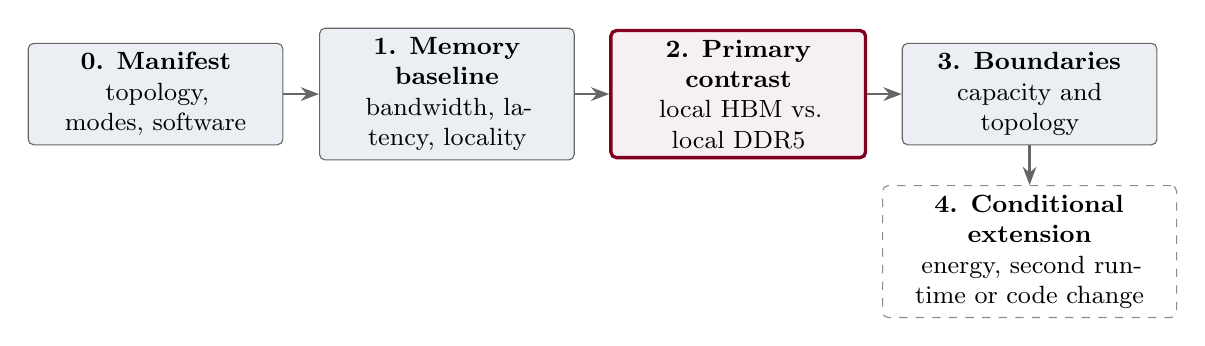
\begin{tikzpicture}[
  font=\small,
  stage/.style={draw=black!60, fill=neutralcol, rounded corners=2pt,
                text width=3.0cm, minimum height=1.15cm, align=center},
  primary/.style={stage, draw=accent, very thick, fill=accent!6},
  optional/.style={draw=black!45, dashed, fill=white, rounded corners=2pt,
                   text width=3.5cm, minimum height=0.95cm, align=center},
  flow/.style={-{Stealth}, thick, black!60}
]
  \node[stage] (s0) at (0,0)
    {\textbf{0. Manifest}\\topology, modes, software};
  \node[stage] (s1) at (3.7,0)
    {\textbf{1. Memory baseline}\\bandwidth, latency, locality};
  \node[primary] (s2) at (7.4,0)
    {\textbf{2. Primary contrast}\\local HBM vs.\ local DDR5};
  \node[stage] (s3) at (11.1,0)
    {\textbf{3. Boundaries}\\capacity and topology};
  \node[optional] (s4) at (11.1,-2.0)
    {\textbf{4. Conditional extension}\\energy, second runtime or code change};

  \draw[flow] (s0) -- (s1);
  \draw[flow] (s1) -- (s2);
  \draw[flow] (s2) -- (s3);
  \draw[flow] (s3) -- (s4);
\end{tikzpicture}
\caption{Experimental dependency order.  The primary HBM--DDR result
does not depend on a later implementation contribution.  Author's
design.}
\label{fig:experimental-sequence}
\end{figure}

\begin{description}
  \item[Stage 0: system manifest.] Record the items in
  Table~\ref{tab:platform-record}, identify HBM and DDR NUMA nodes, and
  verify whether Flat/Cache and Quadrant/SNC4 settings are available.

  \item[Stage 1: memory characterization.] Measure local and remote read,
  copy and triad bandwidth; unloaded and loaded latency; core-count
  scaling; and concurrent HBM--DDR traffic.  Establish saturation and
  run-to-run variability before fitting a performance model.

  \item[Stage 2: primary inference contrast.] Freeze one runtime commit,
  compiler and build.  Separate prefill from decode and compare verified
  local HBM with local DDR5 on one socket.  This stage is the minimum
  complete empirical study.

  \item[Stage 3: capacity and topology.] Move the live set through the
  local HBM boundary, then compare explicit placement, two-socket
  execution and SNC4 where available.  Cache mode is included only if a
  controlled reboot/configuration can be arranged.

  \item[Stage 4: conditional extension.] Add energy, a second runtime or
  a software change only after the baseline identifies a repeatable
  effect and the remaining time supports a proper evaluation.
\end{description}

\subsection{Selecting factors without a Cartesian explosion}

The experiment matrix should be chosen from hypotheses and pilot data,
not by taking every combination of model, precision, length, batch,
core count and topology.

\begin{table}[tbp]
\centering
\small
\caption{Factors and the role of each in the experimental design.}
\label{tab:experimental-factors}
\begin{tabularx}{\textwidth}{@{}lYY@{}}
\toprule
\textbf{Factor} & \textbf{Primary levels} & \textbf{Purpose} \\
\midrule
Memory placement
 & Local HBM and local DDR5; remote and mixed placement in a later stage
 & Isolate tier bandwidth, then quantify locality and spill effects. \\
Working-set regime
 & Comfortably below, near, and above usable local HBM capacity
 & Locate a capacity boundary using measured resident memory rather than
   parameter count alone. \\
Precision
 & BF16 reference and at least one practical quantized weight format;
   KV precision recorded independently
 & Test whether reduced traffic, packing and kernel coverage change the
   HBM benefit. \\
Workload shape
 & Short and long prompt; short and sustained generation; low and
   moderate batch/concurrency
 & Separate prefill, weight-streaming decode and KV-dominant regimes. \\
Core/topology
 & Partial socket, full local socket, two local replicas or an explicit
   shard; SNC4 only if available
 & Identify saturation and distinguish additional compute from remote
   traffic. \\
Cache state
 & Cold-start/model-load and warmed steady state reported separately
 & Prevent file I/O or page-cache state from contaminating inference
   measurements. \\
\bottomrule
\end{tabularx}
\end{table}

Models should be selected by memory regime and architecture rather than
popularity alone.  The design should include a model/format that fits
comfortably in local HBM and one configuration close to the usable
capacity boundary.  At least one grouped-query model is useful because
its KV growth differs from full multi-head attention.  If the boundary
cannot be crossed with available models, context, concurrency or a
controlled allocation can be used to change the live set, provided the
mechanism does not alter the computation being compared.

Pilot runs determine the final numeric levels.  A sparse matrix of
representative points followed by focused sweeps around observed knees
is more informative than a large under-replicated grid.

\subsection{Runtime and correctness controls}

One runtime should be selected as the primary implementation and frozen
at a named commit.  Selection criteria are support for the required
model formats, a measurable prefill/decode boundary, controllable thread
affinity, transparent build reproducibility and a viable way to direct
or verify memory placement.  A second runtime is useful for external
validity but should not multiply every factor in the main experiment.

Performance comparisons are meaningful only when the computation is
equivalent.  Record the model revision and tokenizer, use fixed prompts
and seeds where supported, and validate token sequences or task-level
quality when precision changes.  If different kernels or quantization
formats change model quality, report that difference rather than
treating them as interchangeable.

\subsection{Metrics and explanatory measurements}

The primary metrics are:

\begin{itemize}
  \item prefill-dominated time to first output token (TTFT), with the
        timed boundary declared;
  \item median, p95 and p99 inter-token latency for decode;
  \item output tokens/s and requests/s at the declared concurrency; and
  \item peak and steady resident memory by object or tier where the
        runtime exposes it.
\end{itemize}

E2E latency should be reported with an explicit boundary.  Model loading
and tokenization are measured separately unless the experiment is
deliberately end-to-end.  Throughput and reciprocal latency from the
same fixed synchronous batch are two presentations of one observation,
not independent confirmation.

To explain a result, collect the smallest counter set that can test the
mechanism: HBM and DDR traffic, UPI or remote traffic, achieved
frequency, cache misses and relevant matrix-engine activity.  Counter
names and availability are processor- and permission-specific.  A
counter should be omitted rather than assigned a meaning that its scope
does not support.

\subsection{Run protocol and statistical analysis}

Each reported comparison should follow the same protocol:

\begin{enumerate}
  \item reserve an exclusive node and archive the system manifest;
  \item pin physical cores and memory explicitly, with SMT treated as a
        separate factor;
  \item verify page residency after model initialization and during the
        run, not only after allocation;
  \item separate model loading and warm-up from steady-state timing,
        unless they are part of the declared metric;
  \item counterbalance or randomize HBM and DDR run order to reduce
        thermal and temporal bias;
  \item retain every raw sample, failure and outlier flag together with
        the command and environment;
  \item determine replication from pilot variability, using paired runs
        on the same node where possible; and
  \item repeat a subset on more than one HBM node before generalizing to
        the partition.
\end{enumerate}

Report absolute values and paired effect sizes, not only normalized bar
charts.  For primary comparisons, provide the median and interquartile
range together with a 95\% confidence interval appropriate to the
sampling design.  Tail percentiles require enough generated tokens or
requests to estimate them; p99 from a handful of observations is not a
tail-latency result.

\subsection{Energy, if the boundary can be defended}

RAPL estimates processor-domain energy; XClarity/INA226 and a rack or
node power meter may cover different hardware.  Before reporting
joules/token, validate access, units, update rate, counter wraparound and
the components included in each source.  Integrate energy over the same
timed region as performance.  Gross joules/request and
joules/output-token should be reported; if idle energy is subtracted,
also report the gross value and the subtraction procedure.  Facility
cooling claims require a measured facility boundary and are outside a
node-level study.

\subsection{Threats to validity}

\begin{table}[tbp]
\centering
\small
\caption{Main validity threats and design responses.}
\label{tab:validity}
\begin{tabularx}{\textwidth}{@{}lYY@{}}
\toprule
\textbf{Validity} & \textbf{Threat} & \textbf{Response} \\
\midrule
Internal
 & Frequency drift, first touch, page migration, remote access, warm
   cache state or shared-node interference is mistaken for an HBM effect.
 & Exclusive nodes, paired order, explicit binding, residency checks and
   frequency/traffic measurements. \\
Construct
 & STREAM is treated as LLM bandwidth; file size as live memory; average
   TPOT as tail latency; RAPL as whole-node energy.
 & Define each metric and boundary, measure the live set, and use
   counters only to test a stated mechanism. \\
External
 & One model, precision, node or runtime is generalized to CPU inference
   as a whole.
 & Cover distinct memory regimes, repeat on multiple nodes, and state the
   platform/runtime boundary of every conclusion. \\
Statistical conclusion
 & Few repetitions, selected best runs or unreported failures inflate an
   effect.
 & Retain raw samples, predeclare primary comparisons and report
   uncertainty with absolute values. \\
Reproducibility
 & Modules, firmware, models and scheduler inventory change over time.
 & Archive immutable source/model revisions, build metadata, commands
   and dated system manifests. \\
\bottomrule
\end{tabularx}
\end{table}

\FloatBarrier

\subsection{When an implementation contribution is justified}

The empirical study is complete without a new placement algorithm.  A
software contribution should follow only if the baseline reveals a
stable inefficiency, such as remote pages under an ostensibly local
policy, an avoidable capacity spill, or poor use of the second socket.
The smallest defensible intervention is preferable: separate
HBM/DDR allocators, object-level placement, one worker per locality
domain, or a topology-aware request router.

Any intervention must be compared with strong static baselines,
including all-local placement when the model fits, weights-first and
KV-first tiering, independent per-socket replicas, and hardware Cache
mode if available.  Its evaluation must include placement overhead,
remote traffic, memory use and output quality.  Novelty should be
claimed only after a current literature search and an evaluation show
that the measured advantage is not already provided by an existing
runtime.  It must also distinguish an implemented contribution from the
unevaluated NUMA-aware placement proposed by Na et al.
~\cite{na2024llmcpu}.


\clearpage
\bibliographystyle{plainnat}
\bibliography{../../thesis/references}

\end{document}
